\documentclass[11pt,a4paper]{article}

% ===== EARLY MACROS ================================================
\usepackage[dvipsnames]{xcolor}
\definecolor{accent2}{HTML}{8B0000}
\definecolor{ph}{HTML}{6B7280}

\newcommand{\TODO}[1]{\textcolor{accent2}{\textbf{[TODO: #1]}}}
\newcommand{\phh}[1]{\textcolor{ph}{\textit{*#1}}}

% ===== CONFIGURATION ===============================================
\newcommand{\teamname}{The Three Musketeers}
\newcommand{\topicchoice}{Topic 3 -- AI News Briefing Service}
\newcommand{\member}[2]{\textbf{#1} (#2)}
\newcommand{\reportdate}{September 19, 2026}
\newcommand{\repolink}{\url{https://github.com/aliasefoglu/Final_Project_01/}}

\newcommand{\coursecode}{AI-ENG-110}
\newcommand{\coursename}{Software Engineering}
\newcommand{\institution}{AI Academy, National AI Center}
\newcommand{\semester}{Spring 2026}

% ===== PACKAGES ====================================================
\usepackage[margin=2.2cm,headheight=15pt]{geometry}
\usepackage[T1]{fontenc}
\usepackage[utf8]{inputenc}
\usepackage[final,protrusion=true,expansion=false]{microtype}
\usepackage{amsmath,amssymb}
\usepackage{graphicx}
\usepackage{tikz}
\usetikzlibrary{shapes.geometric,arrows.meta,positioning}
\usepackage{booktabs}
\usepackage{array}
\usepackage{tabularx}
\usepackage{ragged2e}
\usepackage{enumitem}
\usepackage[parfill]{parskip}
\usepackage{listings}
\usepackage[most]{tcolorbox}
\usepackage{titlesec}
\usepackage{fancyhdr}
\usepackage{lastpage}
\usepackage[hidelinks]{hyperref}

\emergencystretch=3em
\hbadness=10000
\hfuzz=2pt

\hypersetup{
  colorlinks=true,
  linkcolor=NavyBlue,
  urlcolor=NavyBlue,
  citecolor=NavyBlue
}

% ===== STYLING =====================================================
\definecolor{accent}{HTML}{0B3D91}
\definecolor{soft}{HTML}{F2F4F8}
\definecolor{deliver}{HTML}{E8F0FE}
\definecolor{deliverframe}{HTML}{1A56DB}
\definecolor{probe}{HTML}{FFF8E1}
\definecolor{probeframe}{HTML}{B45309}

\titleformat{\section}
  {\Large\bfseries\color{accent}}
  {\thesection.}{0.6em}{}

\titleformat{\subsection}
  {\large\bfseries\color{accent}}
  {\thesubsection}{0.5em}{}

\newcommand{\ans}[1]{\rule[-2pt]{#1}{0.5pt}}
\let\ph\phh

\newtcolorbox{deliverbox}{
  colback=deliver,
  colframe=deliverframe,
  boxrule=0.5pt,
  arc=2pt,
  left=8pt,
  right=8pt,
  top=4pt,
  bottom=4pt
}

\newtcolorbox{probebox}{
  colback=probe,
  colframe=probeframe,
  boxrule=0.5pt,
  arc=2pt,
  left=8pt,
  right=8pt,
  top=4pt,
  bottom=4pt
}

\newcommand{\answerbox}[1]{%
  \par\noindent
  \fcolorbox{black!30}{soft}{%
    \parbox{\dimexpr\linewidth-2\fboxsep-2\fboxrule\relax}{%
      \vspace{0pt}\centering
      \ph{[Your response here -- replace this placeholder.]}
      \vspace{#1}
    }%
  }\par
}

\newcommand{\figureplaceholder}[1]{%
  \par\noindent
  \begin{center}
  \fcolorbox{black!30}{soft}{%
    \parbox{0.75\linewidth}{%
      \vspace{0pt}\centering
      \ph{[Replace this box with \texttt{\textbackslash includegraphics\{...\}} or a tikzpicture.]}
      \vspace{#1}
    }%
  }
  \end{center}
}

\definecolor{codegreen}{rgb}{0,0.55,0}
\definecolor{codegray}{rgb}{0.4,0.4,0.4}
\definecolor{codepurple}{rgb}{0.55,0,0.78}
\definecolor{backcolour}{rgb}{0.97,0.97,0.97}

\lstdefinestyle{python}{
  language=Python,
  backgroundcolor=\color{backcolour},
  commentstyle=\color{codegreen},
  keywordstyle=\color{accent},
  numberstyle=\tiny\color{codegray},
  stringstyle=\color{codepurple},
  basicstyle=\ttfamily\footnotesize,
  breakatwhitespace=false,
  breaklines=true,
  keepspaces=true,
  numbers=left,
  numbersep=6pt,
  tabsize=2,
  frame=single,
  framerule=0.4pt,
  rulecolor=\color{black!30},
}

\pagestyle{fancy}
\fancyhf{}
\fancyhead[L]{\small\textit{*\coursecode\ -- Final Report -- \teamname}}
\fancyhead[R]{\small\textit{*\semester}}
\fancyfoot[L]{\small\textit{*\institution}}
\fancyfoot[R]{\small Page \thepage\ of \pageref{LastPage}}
\renewcommand{\headrulewidth}{0.4pt}
\renewcommand{\footrulewidth}{0.4pt}

% ===================================================================
\begin{document}

\begin{center}
{\small
\textsc{\institution}\\[0.2em]
\textsc{\coursecode\ -- \coursename\ -- \semester}
}\\[1.2em]

{\Large\bfseries\color{accent} Final Project Report}\\[0.3em]

{\LARGE\bfseries \topicchoice}\\[0.6em]

\rule{0.85\textwidth}{0.6pt}
\end{center}

\vspace{0.6em}

\begin{tabularx}{\textwidth}{@{}lXlX@{}}
\textbf{Team:} & \teamname &
\textbf{Date:} & \reportdate \\

\textbf{Repo:} & \repolink &
\textbf{Tag:} & \texttt{v1.0-final} \\

\textbf{Members:} &
\multicolumn{3}{X@{}}{
  \member{Ali Huseynli}{@aliasefoglu},\quad
  \member{Alish Hajiyev}{@alishhajiyev},\quad
  \member{Elsen Samadzada}{@elshansamadzada7}
}
\\
\end{tabularx}

\vspace{0.4em}
\hrule
\vspace{0.6em}

% ===================================================================
\section*{Executive Summary}
\addcontentsline{toc}{section}{Executive Summary}


We built \texttt{NewsBrief}, a service that collects articles from several news sources, removes duplicate stories, summarizes the remaining articles, and creates a personalized Markdown digest for each user. The system uses six configured sources, PostgreSQL for persistent data and caching, and the course-provided AI package for summarization and topic labeling. For a benchmark of 20 fetch operations, the concurrent implementation finished in 3.00 seconds, compared with 13.79 seconds for the sequential version, which corresponds to a 4.6$\times$ speedup. We also tested the system against a real failure during development: the Reuters HTML source returned HTTP 401 responses, but the failure was isolated to that source and the other sources continued normally. Another important lesson was that database design required more work than we expected, especially when we changed the user's topic list from JSONB to normalized relational tables. If we continued the project, we would add source-health tracking, a shared provider-rate-limit mechanism, and an integration test using the real PostgreSQL container.

% ===================================================================
\tableofcontents

\vspace{0.6em}
\hrule
\vspace{0.4em}

% ===================================================================
\section{Project Overview}

\subsection{Problem framing \& scope}


The main purpose of the system is to collect recent news for a user, remove repeated coverage of the same story, summarize the remaining articles, and produce a short personalized briefing. Articles are collected from RSS feeds and one HTML-scraped source. After fetching, the system performs URL/content normalization and near-duplicate detection before sending new content to the AI service. The final digest is stored as a Markdown file under \texttt{digests/}.

There are two user-facing entry points. The main one is the CLI command \texttt{python -m src.cli run-daily --user <name>}. We also implemented a small FastAPI web application in \texttt{src/api.py}, which provides signup, login, topic preferences, and access to the latest digest. The web interface was added as an extension to the required CLI workflow so that the project could also be demonstrated through a browser.

The configured LLM provider is Google Gemini, using \texttt{LLM\_PROVIDER=google} and the model \texttt{gemini-3.6-flash}. We do not use the embedding provider. The two required deduplication stages are sufficient for the current implementation, so adding embeddings would not provide a necessary function in the pipeline.

We also chose not to add semantic clustering based on embeddings. The specification provides embeddings as an available AI primitive, but the required URL/content and near-duplicate stages already give us the duplicate filtering needed for this project. Instead, we spent the available development time on the fetch layer, database design, testing, and the additional web interface.

% ===================================================================
\subsection{Provider choice and the AI module contract}


We use Google Gemini through the provider factory supplied by the course package. The configured model is \texttt{gemini-3.6-flash}. No embedding model is used. Our code calls \texttt{ai.summarize\_and\_label} from \texttt{src/services/ai\_service.py}; this is the only direct call from our service layer into the provided AI package.

We did not modify any file inside \texttt{ai/}. The application-specific code is located under \texttt{src/}, while the supplied package remains unchanged.

The provided AI package validates the returned data against its \texttt{LabeledSummary} schema. This means that invalid enum values or other schema violations are rejected before a result is returned to our service layer. Provider errors are handled separately by \texttt{AIService}, which retries transient provider failures. When the retry limit is reached, the pipeline records the failure for that article and continues with the other articles.

% ===================================================================
\section{Architecture}\label{sec:arch}

\subsection{Module map}

\begin{center}
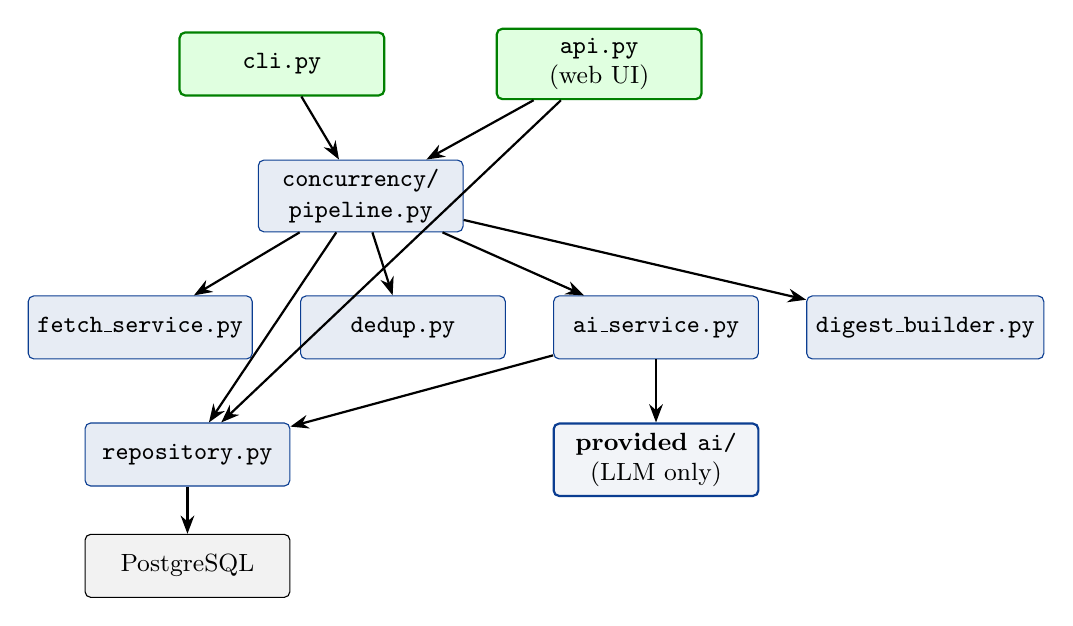
\begin{tikzpicture}[
  node distance=4mm,
  box/.style={
    draw,
    rounded corners=2pt,
    minimum width=2.6cm,
    minimum height=0.8cm,
    align=center,
    font=\small
  },
  aibox/.style={
    box,
    fill=soft,
    draw=accent,
    thick
  },
  sebox/.style={
    box,
    fill=accent!10,
    draw=accent
  },
  entry/.style={
    box,
    fill=green!12,
    draw=green!50!black,
    thick
  },
  arrow/.style={-Stealth,thick}
]

  \node[entry] (cli) {\texttt{cli.py}};
  \node[entry,right=14mm of cli] (api) {\texttt{api.py}\\(web UI)};

  \node[sebox,below=8mm of cli,xshift=10mm]
    (pipe) {\texttt{concurrency/}\\\texttt{pipeline.py}};

  \node[sebox,below=8mm of pipe,xshift=-28mm]
    (fetch) {\texttt{fetch\_service.py}};

  \node[sebox,right=6mm of fetch]
    (dedup) {\texttt{dedup.py}};

  \node[sebox,right=6mm of dedup]
    (aisvc) {\texttt{ai\_service.py}};

  \node[sebox,right=6mm of aisvc]
    (digest) {\texttt{digest\_builder.py}};

  \node[aibox,below=8mm of aisvc]
    (ai) {\textbf{provided \texttt{ai/}}\\(LLM only)};

  \node[sebox,below=8mm of fetch,xshift=6mm]
    (repo) {\texttt{repository.py}};

  \node[box,below=6mm of repo,fill=gray!10]
    (pg) {PostgreSQL};

  \draw[arrow] (cli) -- (pipe);
  \draw[arrow] (api) -- (pipe);
  \draw[arrow] (pipe) -- (fetch);
  \draw[arrow] (pipe) -- (dedup);
  \draw[arrow] (pipe) -- (aisvc);
  \draw[arrow] (pipe) -- (digest);
  \draw[arrow] (aisvc) -- (ai);
  \draw[arrow] (pipe) -- (repo);
  \draw[arrow] (aisvc) -- (repo);
  \draw[arrow] (api) -- (repo);
  \draw[arrow] (repo) -- (pg);

\end{tikzpicture}
\end{center}

The two entry points are \texttt{cli.py} and \texttt{api.py}. Both use the pipeline in \texttt{concurrency/pipeline.py}. The pipeline coordinates fetching, deduplication, AI processing, digest creation, and persistence.

\texttt{services/fetch\_service.py} is responsible for retrieving articles. \texttt{core/dedup.py} performs normalization and duplicate detection. \texttt{services/ai\_service.py} is the only application module that directly communicates with the supplied \texttt{ai/} package. \texttt{core/digest\_builder.py} creates the final Markdown output. Database access is kept in \texttt{storage/repository.py}, while PostgreSQL contains the persistent user, preference, account, and processed-content data.

% ===================================================================
\subsection{OOP design \& key abstractions}


\begin{lstlisting}[style=python]
class NewsSource(abc.ABC):
    """Common interface for configured news sources."""
    name: str

    @abc.abstractmethod
    async def fetch(
        self, client: httpx.AsyncClient
    ) -> list[Article]:
        raise NotImplementedError


@dataclass
class RssSource(NewsSource):
    feed_url: str
    name: str = ""

    async def fetch(
        self, client: httpx.AsyncClient
    ) -> list[Article]:
        ...
\end{lstlisting}

We use \texttt{NewsSource} as an abstract base class because RSS and HTML sources have different fetching implementations but expose the same operation to the rest of the application. The pipeline therefore does not need to know which concrete source it is using. The common contract also makes it straightforward to add another source without changing the orchestration code.

We use composition in other parts of the system. For example, \texttt{AIService} and \texttt{Deduplicator} are separate components used by the pipeline rather than subclasses of a common base class. There is no useful type hierarchy between them, so composition keeps the responsibilities separate.

% ===================================================================
\subsection{Data flow across module boundaries}

Our application models in \texttt{src/models.py} include \texttt{Article}, \texttt{LabeledSummary}, \texttt{Source}, \texttt{ProcessedArticle}, \texttt{BriefingItem}, \texttt{User}, and \texttt{Account}. These models define the data passed between the main application components.

We do not use unstructured dictionaries as the normal interface between modules. The exception is the internal \texttt{DigestItem} helper in \texttt{core/digest\_builder.py}, which is only used while constructing the final digest and is never stored or sent across an external service boundary.

The models supplied by \texttt{ai/} are used only around the AI call. Our own \texttt{Article} model contains application-specific fields such as \texttt{id}, \texttt{canonical\_url}, and \texttt{content\_hash}, which are needed by fetching, deduplication, and storage. The conversion between the two model sets is kept in \texttt{ai\_service.py}.

% ===================================================================
\section{Concurrency \& Performance}\label{sec:concurrency}

\subsection{Why this concurrency model}

The fetch layer uses \texttt{asyncio} together with \texttt{httpx.AsyncClient}. Fetching articles is mainly an I/O-bound task because the application spends most of its time waiting for remote servers to respond. Using asynchronous requests allows several sources to be processed while other requests are waiting.

The maximum number of concurrent fetches is controlled by \texttt{MAX\_PARALLEL\_FETCHES}, which is set to 8 by default. This value follows the project specification and is large enough for the configured sources without creating an unnecessarily large number of simultaneous requests.

A thread pool could also handle network requests, but it would introduce thread management without providing a clear advantage for this workload. With asyncio, the concurrency is explicit in the source-fetching code and works naturally with the existing asynchronous HTTP client.

When the semaphore is set to 1, requests are effectively processed one at a time, so the implementation approaches the sequential case. Increasing the value above the number of independent source tasks does not provide additional benefit. For the current six-source configuration, a limit of 100 therefore does not mean that 100 requests will be executed at once.

% ===================================================================
\subsection{Sequential-vs-concurrent benchmark}

\begin{center}
\small
\begin{tabular}{lcccc}
\toprule
\textbf{Workload} &
$N$ &
\textbf{Sequential (s)} &
\textbf{Concurrent (s)} &
\textbf{Speedup} \\
\midrule
fetch (\texttt{scripts/bench.py}) &
20 &
13.79 &
3.00 &
4.6$\times$ \\
\bottomrule
\end{tabular}
\end{center}

The benchmark used 20 fetch operations and a maximum concurrency of 8. The sequential version took 13.79 seconds, while the concurrent version took 3.00 seconds. This gives a measured speedup of approximately 4.6$\times$.

The result is lower than an ideal 8$\times$ improvement because the requests do not all take the same amount of time and because the six configured sources limit the amount of useful source-level parallelism. The Reuters source also failed during the benchmark and went through its retry logic, which added additional waiting time.

% ===================================================================
\subsection{Rate limit \& politeness}

The fetch layer uses \texttt{tenacity} to retry temporary HTTP and transport failures. Each request can be attempted up to three times with exponential backoff. Fetch concurrency is separately limited by \texttt{Semaphore(MAX\_PARALLEL\_FETCHES=8)}.

The AI layer has its own retry policy. Provider errors can be retried up to four times with exponential backoff, with the delay capped at 20 seconds. These two mechanisms are separate because HTTP fetching and LLM requests have different failure conditions.

During development, we observed real Gemini quota errors. The free-tier configuration returned HTTP 429 responses after the request limits were reached. The logged error included \texttt{RESOURCE\_EXHAUSTED} and indicated the daily free-tier request quota. Once the daily quota was exhausted, retrying could not restore the request capacity, so the affected articles were skipped and the pipeline continued.

To reduce unnecessary requests during development, we added \texttt{AI\_DRY\_RUN} and \texttt{MAX\_ARTICLES\_PER\_RUN}. These settings allowed the rest of the pipeline to be tested without repeatedly consuming the available LLM quota.

% ===================================================================
\section{Robustness \& Error Handling}\label{sec:robustness}

\subsection{Wrapping the AI module}

\texttt{AIService} in \texttt{src/services/ai\_service.py} is the single application-level wrapper around \texttt{ai.summarize\_and\_label}. Provider errors are retried four times using exponential backoff, with a maximum delay of 20 seconds. Other exceptions are not automatically retried because they may represent deterministic application errors rather than temporary provider problems.

The supplied AI function is synchronous, so our service executes it through \texttt{asyncio.to\_thread} and places a 30-second timeout around the operation. This prevents one slow provider call from blocking the rest of the asynchronous pipeline indefinitely.

The service logs the article title and a short prefix of the content hash. Retry attempts are logged at warning level. The full article content is not written to the logs.

Before the AI call, the article must already have a content hash produced by the deduplication stage. The returned object is validated by the supplied AI package. Successfully validated summaries are then stored in the database and can be reused on later runs.

% ===================================================================
\subsection{Failure-mode analysis (one concrete incident)}

The most concrete failure observed during the benchmark was the HTML-scraping source returning HTTP 401 responses from Reuters. This occurred during the real \texttt{scripts/bench.py --N 20} benchmark rather than through an artificial test injection.

The fetch function retried the request three times. After the retries were exhausted, the exception was caught at the source level. The source was logged as failed and returned no articles, while the remaining RSS sources continued processing.

From the user's perspective, the run still completed and produced its output. The failed source did not terminate the complete pipeline. The log contained the HTTP 401 error and the message indicating that the source was skipped after the retry attempts.

The incident also exposed a limitation. The application does not currently distinguish between a temporary source failure and a source that has been unavailable for a long period. As a result, the same source can consume retry attempts on every future run until its URL or configuration is changed.

% ===================================================================
\subsection{Input validation}

The CLI requires the \texttt{--user} argument through \texttt{argparse}. The current implementation does not apply an additional username-format restriction.

The web interface checks that usernames are not empty, passwords contain at least eight characters, and password confirmation matches the original password. Login failures use the same generic error message for an unknown username and an incorrect password.

Fetched RSS entries without a title or link are ignored. HTML pages are also skipped when the required title or article text cannot be extracted. URLs and article content are normalized before they enter the deduplication process. Valid data is then represented using the application's typed models.

One current limitation is in the topic-preference form. The submitted values are converted directly to \texttt{TopicEnum}; an invalid topic value submitted outside the normal browser form can therefore result in a \texttt{ValueError}. This should be converted into controlled validation handling before a production deployment.

% ===================================================================
\section{Storage \& Caching}\label{sec:storage}

\subsection{Schema}

\begin{lstlisting}[style=python,language=sql,numbers=none,basicstyle=\ttfamily\footnotesize]
CREATE TABLE users (
    user_id          TEXT PRIMARY KEY,
    preferred_length TEXT NOT NULL DEFAULT 'medium'
                     CHECK (preferred_length IN ('short','medium','long'))
);

CREATE TABLE user_preferred_topics (
    user_id TEXT NOT NULL
            REFERENCES users(user_id) ON DELETE CASCADE,
    topic   TEXT NOT NULL
            CHECK (topic IN ('Politics','Tech','Sports',
                             'Business','Health','Science',
                             'World','Entertainment','Other')),
    PRIMARY KEY (user_id, topic)
);

CREATE TABLE user_excluded_sources (
    user_id TEXT NOT NULL
            REFERENCES users(user_id) ON DELETE CASCADE,
    source  TEXT NOT NULL,
    PRIMARY KEY (user_id, source)
);

CREATE TABLE accounts (
    user_id       TEXT PRIMARY KEY
                  REFERENCES users(user_id) ON DELETE CASCADE,
    password_hash TEXT NOT NULL,
    created_at    TIMESTAMPTZ NOT NULL DEFAULT now()
);

CREATE TABLE processed_urls (
    content_hash  CHAR(64) PRIMARY KEY,
    canonical_url TEXT NOT NULL UNIQUE,
    summary       TEXT,
    topic         TEXT,
    sentiment     TEXT,
    processed_at  TIMESTAMPTZ NOT NULL DEFAULT now()
);
\end{lstlisting}

The database uses separate tables for user topics and excluded sources instead of storing lists inside the \texttt{users} table. This keeps individual values atomic and makes the schema easier to query. Foreign keys with \texttt{ON DELETE CASCADE} also ensure that related preference and account records are removed when the corresponding user is deleted.

User information and preferences are source-of-truth data. The \texttt{processed\_urls} table stores derived AI results and is used as the application's persistent summary cache.

User updates are performed inside an explicit database transaction. This means that changes affecting several related tables are either committed together or rolled back together.

% ===================================================================
\subsection{Caching policy}

The application caches the AI result for an article using its SHA-256 content hash. The result is stored in \texttt{processed\_urls}. When an article with the same content hash is encountered again, the existing result can be used without another LLM request.

There is no time-based cache expiration. The reason is that the cache key is based on the normalized article content rather than only the URL. If the content changes, the hash changes and the application treats it as new content.

The main case where an old result could become outdated is a change in the AI prompt or model. A summary generated by one model would remain associated with the same content hash even after a model change. A production version could include a model or prompt version in the cache key.

A numerical cache-hit percentage is not included because the current project evidence does not contain a reproducible hit/miss count from one complete demo run. The existing logs distinguish cache hits from fresh AI calls, so the percentage can be measured directly from a controlled two-run test.

% ===================================================================
\section{Testing}\label{sec:testing}

\subsection{Strategy \& coverage}

The application tests do not call the real LLM provider. The pipeline tests use a fake \texttt{AIService} and a fake repository, while asynchronous operations are controlled with \texttt{AsyncMock} and \texttt{monkeypatch}. HTTP requests are intercepted with \texttt{respx}, so the fetch tests do not depend on external websites.

The full test suite contains 69 passing tests in the Docker environment. The supplied AI smoke tests also pass.

\begin{center}
\small
\begin{tabular}{lc}
\toprule
\textbf{Suite} & \textbf{Coverage} \\
\midrule
\texttt{src/} (our SE layer only) & 86.7\% \\
Provided \texttt{ai/} smoke tests & \textcolor{codegreen}{passing (15/15)} \\
\bottomrule
\end{tabular}
\end{center}

The coverage for the application code is 86.7\%. The combined coverage reported by \texttt{pytest-cov} is approximately 90\%, but the more useful number for the project is the coverage of \texttt{src/}, since this is the code written by the team.

For type checking, \texttt{mypy --explicit-package-bases --disable-error-code=import-untyped src} reports no errors in the application code. The remaining reported errors are inside the supplied AI provider files and were not changed because the \texttt{ai/} package is read-only for this project.

% ===================================================================
\subsection{Notable tests}

\textbf{Happy path.}
\texttt{test\_pipeline.py::test\_run\_daily\_pipeline\_happy\_path} runs the main pipeline with controlled fetch, AI, and repository components. It verifies that the expected article appears in the generated digest and that a duplicate containing URL tracking parameters is removed.

\textbf{Concurrency.}
\texttt{test\_fetch.py::test\_fetch\_all\_sources\_runs\_sources\_concurrently} creates three sources and makes one of them raise \texttt{httpx.ConnectError}. The test checks that the other sources still return their articles. This verifies that a single failed source does not terminate the complete fetch operation.

\textbf{Error path.}
\texttt{test\_pipeline.py::test\_run\_daily\_pipeline\_skips\_articles\_that\_fail\_ai\_labeling} forces AI labeling to fail and checks that the pipeline still finishes and writes an appropriate digest. This test is important because an LLM failure should affect the corresponding article rather than terminate the complete daily run.

The main missing test is a real integration test against PostgreSQL. The current storage tests mock \texttt{asyncpg}, which keeps them fast but means that a mismatch between the SQL schema and an actual database could still be missed by unit tests.

% ===================================================================
\section{Deployment \& Reproducibility}\label{sec:deploy}

\subsection{Docker image}

The project is run through Docker Compose. The main build command is:

\begin{lstlisting}[style=python,language=bash,numbers=none]
docker compose up -d --build
\end{lstlisting}

The application consists of the PostgreSQL database, the scheduler/application container, and the FastAPI web service. A single pipeline run can be started with:

\begin{lstlisting}[style=python,language=bash,numbers=none]
docker compose run --rm app \
  python -m src.cli run-daily --user khagani
\end{lstlisting}

The Dockerfile uses \texttt{python:3.12-slim} and a two-stage build. Build dependencies are installed in the builder stage and the resulting Python packages are copied into the runtime stage. This keeps the compiler toolchain out of the final image.

The exact image size was not recorded in the project evidence used for this report, so no specific size is claimed here. It can be obtained from the final build with:

\begin{lstlisting}[style=python,language=bash,numbers=none]
docker images
\end{lstlisting}

% ===================================================================
\subsection{Configuration}

The main configuration values are stored in \texttt{.env} and documented through \texttt{.env.example}.

\begin{itemize}
    \item \texttt{LLM\_PROVIDER}: selects the LLM provider.
    \item \texttt{LLM\_MODEL}: selects the configured model.
    \item The corresponding provider API key: required when the application makes an actual LLM request.
    \item \texttt{DATABASE\_URL}: specifies the PostgreSQL connection. A reachable database is required for normal application operation.
    \item \texttt{HTML\_SCRAPE\_URL}: specifies the HTML source.
    \item \texttt{HTML\_SCRAPE\_SOURCE\_NAME}: gives the configured name of that source.
    \item \texttt{SESSION\_SECRET\_KEY}: used for web sessions. A development default exists, but a real deployment should provide a private value.
    \item \texttt{DEDUP\_NEAR\_DUPLICATE\_THRESHOLD}: controls the near-duplicate threshold.
    \item \texttt{MAX\_PARALLEL\_FETCHES}: controls fetch concurrency and defaults to 8.
    \item \texttt{FETCH\_TIMEOUT\_SECONDS}: controls HTTP request timeouts.
    \item \texttt{LOG\_LEVEL}: controls logging verbosity.
    \item \texttt{DIGESTS\_DIR}: specifies where generated digests are written.
\end{itemize}

Most of the operational settings have defaults, while the database and LLM configuration are required for the corresponding parts of the application to work.

% ===================================================================
\section{Limitations \& Future Work}\label{sec:limits}

\begin{itemize}
\setlength\itemsep{0.4em}

\item
\textbf{HTML scraping is source-dependent.}
The \texttt{HtmlScrapeSource} depends on the current HTML structure of its target website. A change in the page structure can cause the source to return no usable articles until its selectors are updated.

\item
\textbf{There is no secondary LLM provider.}
If the configured provider remains unavailable after the retry attempts, affected articles are skipped. The application does not currently switch automatically to another provider.

\item
\textbf{Topic validation needs stronger handling.}
A manually forged HTTP request containing an invalid topic value can currently result in a \texttt{ValueError}. This should be converted into a controlled validation response.

\item
\textbf{Password hashing could be stronger for production.}
The current implementation uses PBKDF2-HMAC-SHA256. It is suitable for the scope of the coursework and does not require another dependency, but a production authentication system could use a password-hashing library designed specifically for this purpose.

\item
\textbf{There is no shared provider budget across runs.}
The fetch semaphore limits concurrency inside a run, but separate scheduled runs do not share a common LLM request budget. This can become important when multiple users are processed close together.

\end{itemize}

With another week, we would first add a real PostgreSQL integration test and improve validation in the web interface. We would then add source-health tracking so permanently unavailable sources are not retried indefinitely. A shared provider budget would also make scheduled multi-user runs safer with respect to external API limits.

% ===================================================================
\section{Tools \& Acknowledgements}\label{sec:tools}

During development, the team used AI-based tools as supplementary development and writing aids. The project requirements, architecture, implementation choices, testing process, and final technical decisions were reviewed by the team and tested against the actual application.

Claude was used during development to help review parts of the code structure and suggest improvements to selected implementation details. The suggestions were checked against the project requirements and adapted where necessary.

ChatGPT was also used for language support, including improving grammar, organizing explanations, and reviewing parts of the report and presentation text. The final report describes the implementation and test results of the project itself, and the team reviewed the final technical content before submission.

% ===================================================================
\section*{References}
\addcontentsline{toc}{section}{References}

The project references were official documentation for Python \texttt{asyncio}, HTTPX, tenacity, Pydantic, FastAPI, asyncpg, PostgreSQL, Docker Compose, and the Gemini API which was used when implementing and checking framework-specific functionality. Additionally, the Topic 3 specification and the course-provided \texttt{ai/} package was used for this project. 

\begin{enumerate}
[label={[\arabic*]},leftmargin=2.4em,itemsep=2pt]

  \item \texttt{tenacity} documentation:
  \url{https://tenacity.readthedocs.io/}

  \item \texttt{asyncpg} documentation:
  \url{https://magicstack.github.io/asyncpg/current/}

  \item FastAPI documentation:
  \url{https://fastapi.tiangolo.com/}

  \item \texttt{pydantic-settings} documentation:
  \url{https://docs.pydantic.dev/latest/concepts/pydantic_settings/}

  \item PostgreSQL documentation, transactions:
  \url{https://www.postgresql.org/docs/current/tutorial-transactions.html}

  \item Python \texttt{asyncio} documentation:
  \url{https://docs.python.org/3/library/asyncio.html}

  \item HTTPX documentation:
  \url{https://www.python-httpx.org/}

  \item Pydantic documentation:
  \url{https://docs.pydantic.dev/}

  \item Docker Compose documentation:
  \url{https://docs.docker.com/compose/}

  \item Gemini API documentation:
  \url{https://ai.google.dev/gemini-api/docs}

  \item AI-ENG-110 Topic 3 specification (\texttt{TOPIC.md}), AI Academy,
  National AI Center, Spring 2026.

\end{enumerate}


% ===================================================================
\appendix

\section{Appendix --- Reproducing the benchmark}

The benchmark can be reproduced from the repository with the following commands:

\begin{lstlisting}[style=python,language=bash,numbers=none]
git clone <repo>
cd <repo>

cp .env.example .env
# Configure the required provider settings.

docker compose build app

docker compose run --rm app \
  python scripts/bench.py --N 20
\end{lstlisting}

The benchmark compares the sequential and concurrent fetch implementations using the same workload. The reported project result was 13.79 seconds for the sequential run and 3.00 seconds for the concurrent run.

\vspace{1em}
\hrule
\vspace{0.6em}

\noindent
\small\textit{*End of report --- thank you for reading.}

\end{document}